\section{Assignment 10}

\subsection{Design the operational space inverse dynamics control law}

\begin{figure}[H]
\centering
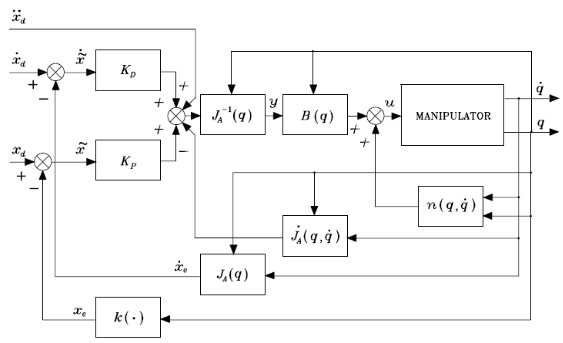
\includegraphics[keepaspectratio,width=0.35\textwidth]{op_inv_arch}
\caption{Operational space inverse dynamics control law architecture}
\end{figure}

The operational space inverse dynamics control law works exactly the same as the joint space one, except for the transformation of the joint space quantities into the corresponding operational space ones with direct kinematics (i.e. with the use of the transformation matrix $T$, the analytical Jacobian $JA$ and its inverse $JA^{-1}$ and derivative $\dot JA$). The control law parameters are $K_P=100,K_D=15$. The architecture was tested with a constant pose reference obtained by applying direct kinematics to the same waypoints seen in the joint space case.

\begin{figure}[H]
\centering
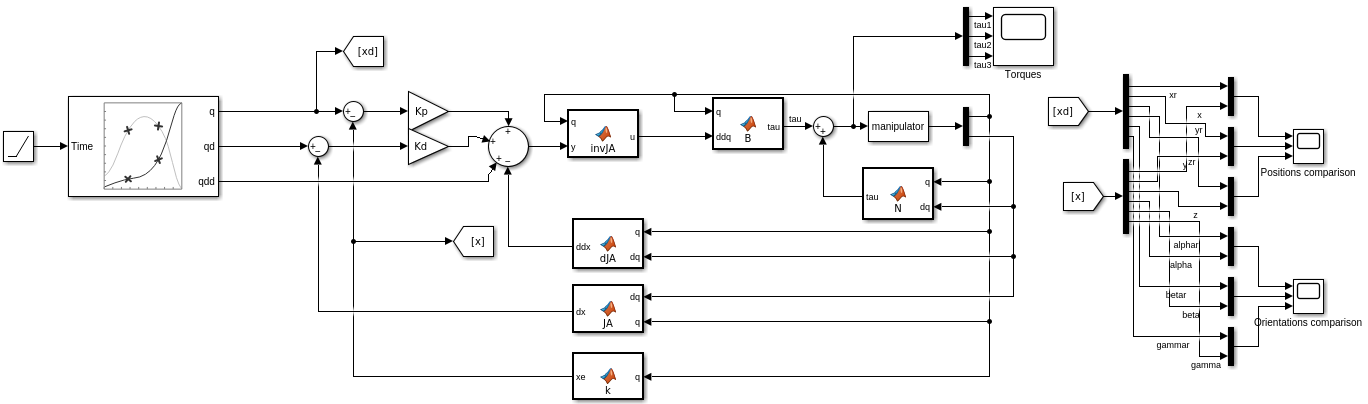
\includegraphics[keepaspectratio,width=0.7\textwidth]{op_inv_sim}
\caption{Operational space inverse dynamics control lawSIMULINK model}
\end{figure}

\begin{figure}[H]
\begin{minipage}{0.5\textwidth}
\centering
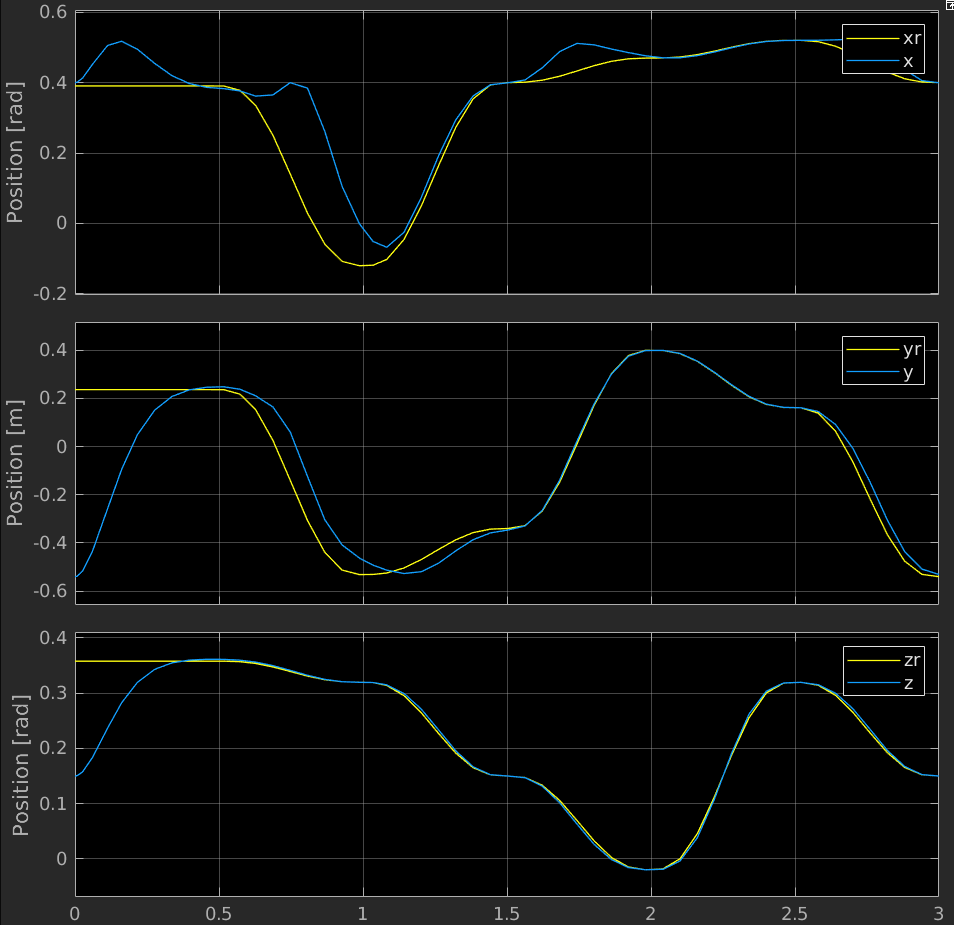
\includegraphics[keepaspectratio,width=\textwidth]{op_inv_pos}
\caption{Pose tracking - end-effector xyz coordinates}
\end{minipage}
\begin{minipage}{0.5\textwidth}
\centering
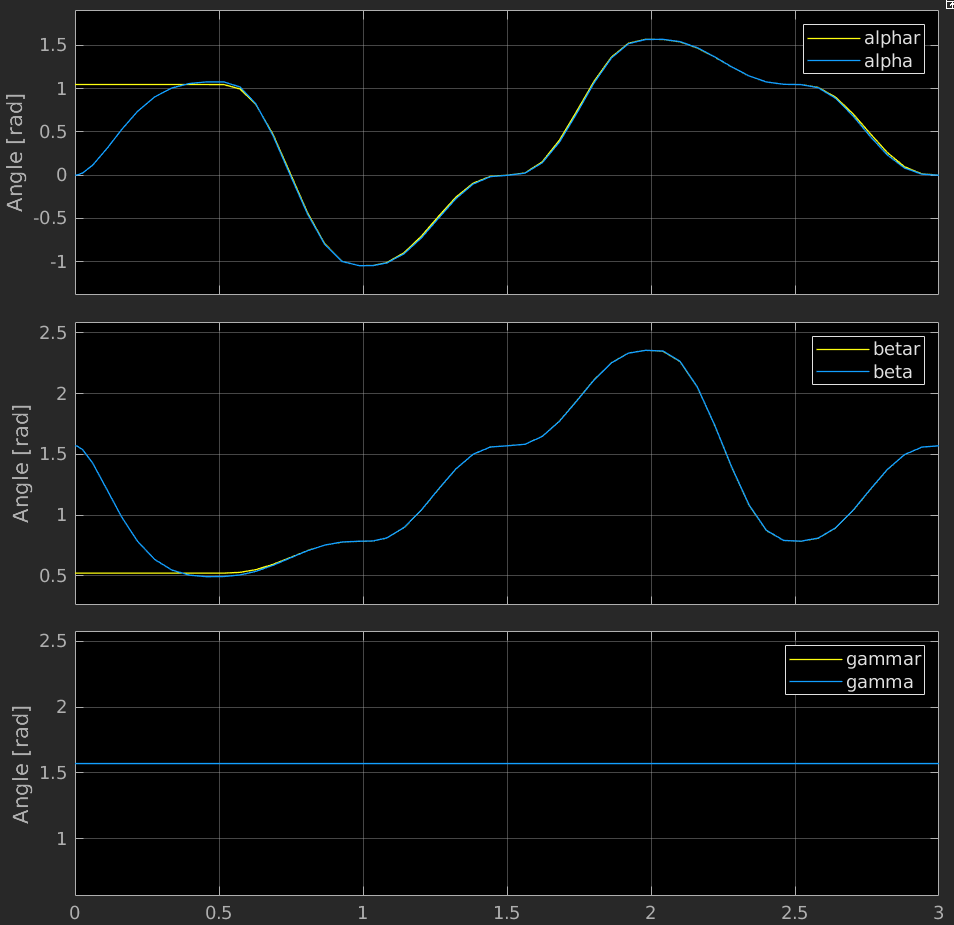
\includegraphics[keepaspectratio,width=\textwidth]{op_inv_or}
\caption{Pose tracking - end-effector $\alpha\beta\gamma$ coordinates}
\end{minipage}
\end{figure}